\documentclass{article}

\usepackage{graphicx}
\usepackage{tikz}
\usepackage{tikzsymbols}
\usetikzlibrary{calc,patterns,shapes.geometric}
\pagestyle{empty}
\usepackage[margin=0pt]{geometry}
\geometry{papersize={14in,12in}}

\def\centerarc[#1](#2)(#3:#4:#5){\draw[#1] ($(#2)+({#5*cos(#3)},{#5*sin(#3)})$) arc (#3:#4:#5);}

\begin{document}
	\begin{figure}
		\centering
		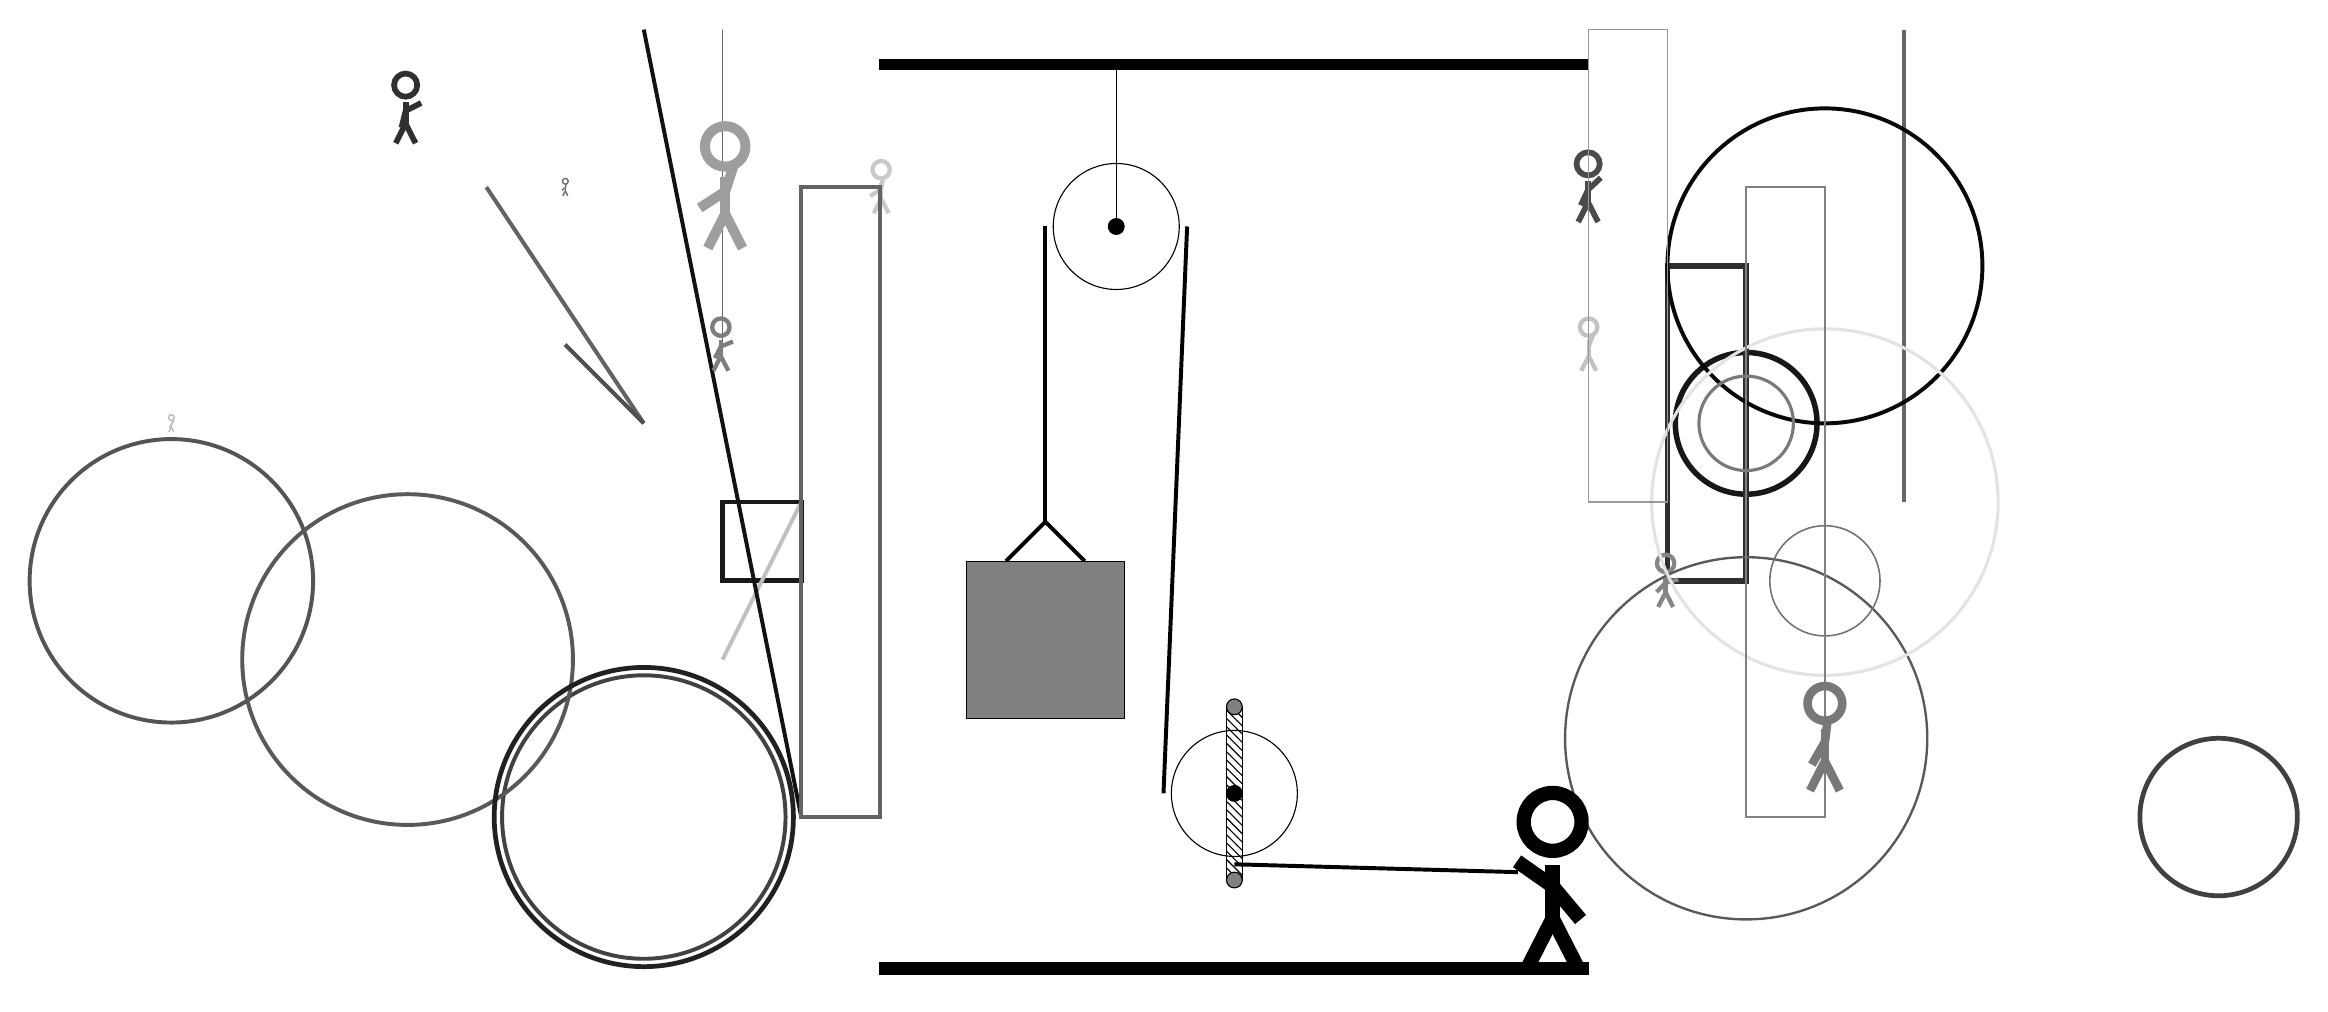
\begin{tikzpicture}
			%%%%% START %%%%%
			
			\draw[fill=black] (-2, 11.5) rectangle (7, 11.625);
			
			\draw (1, 9.5) circle (0.8);
			\draw[fill=black] (1, 9.5) circle (0.1);
			\draw (1, 11.5) -- (1, 9.5);
			
			\node[line width=0.2mm, color=black!24] at (7, 8) {\Strichmaxerl[3][90][69]};
			
			\draw[line width=0.5mm, color=black!61](-7, 10) -- (-5, 7);
			\draw[line width=0.6mm, color=black!90] (-3, 5) rectangle (-4, 6);
			\draw[line width=0.5mm, color=black!60](11, 6) -- (11, 12);
			
			\draw [line width=0.7mm, color=black!91](9, 7) circle (0.9);
			
			\draw [line width=0.6mm, color=black!84](11, 4) circle (0.0);
			\node[line width=0.6mm, color=black!81] at (-8, 11) {\Strichmaxerl[4][76][27]};
			\draw [line width=0.5mm, color=black!74](-5, 2) circle (1.8);
			\draw[line width=0.5mm, color=black!25](-4, 4) -- (-3, 6);
			\node[line width=0.5mm, color=black!21] at (-2, 10) {\Strichmaxerl[3][33][81]};
			
			\draw[line width=0.2mm, color=black!59] (-4, 8) rectangle (-4, 12);
			\draw [line width=0.5mm, color=black!67](-11, 5) circle (1.8);
			\draw [line width=0.6mm, color=black!75](15, 2) circle (1.0);
			
			\draw[line width=0.5mm, color=black!69](-5, 7) -- (-6, 8);
			\node[line width=0.7mm, color=black!27] at (-11, 7) {\Strichmaxerl[1][63][52]};
			\draw[line width=0.5mm, color=black!93](-3, 2) -- (-5, 12);
			
			\draw[line width=0.5mm, color=black!61] (-2, 10) rectangle (-3, 2);
			\draw[line width=0.7mm, color=black!82] (8, 9) rectangle (9, 5);
			\draw [line width=0.5mm, color=black!97](10, 9) circle (2.0);
			
			\draw [line width=0.5mm, color=black!65](-8, 4) circle (2.1);
			\node[line width=0.4mm, color=black!71] at (7, 10) {\Strichmaxerl[4][65][43]};
			
			\draw [line width=0.4mm, color=black!52](9, 7) circle (0.6);
			\node[line width=0.6mm, color=black!48] at (8, 5) {\Strichmaxerl[3][46][14]};
			\node[line width=0.3mm, color=black!38] at (-4, 10) {\Strichmaxerl[7][33][72]};
			\draw [line width=0.3mm, color=black!65](9, 3) circle (2.3);
			
			\draw [line width=0.2mm, color=black!55](10, 5) circle (0.7);
			\draw [line width=0.4mm, color=black!11](10, 6) circle (2.2);
			\draw [line width=0.6mm, color=black!87](-5, 2) circle (1.9);
			
			\draw[line width=0.2mm, color=black!50] (9, 10) rectangle (10, 2);
			\node[line width=0.3mm, color=black!57] at (-6, 10) {\Strichmaxerl[1][38][78]};
			\draw[line width=0.2mm, color=black!40] (7, 12) rectangle (8, 6);
			\node[line width=0.6mm, color=black!51] at (-4, 8) {\Strichmaxerl[3][63][22]};
			\node[line width=0.2mm, color=black!53] at (10, 3) {\Strichmaxerl[6][60][83]};
			
			\draw[fill=white](2.5, 2.3) circle (0.8);
			\draw[fill=black] (2.5, 2.3) circle (0.1);
			\draw[pattern=north west lines, pattern color=black] (2.4, 3.4) rectangle (2.6, 1.2);
			\draw[fill=black!50] (2.5, 3.4) circle (0.1);
			\draw[fill=black!50] (2.5, 1.2) circle (0.1);
			
			\draw[line width=0.5mm] (-0.4, 5.25) -- (0.1, 5.75) -- (0.6, 5.25);
			\draw[fill=black!50] (-0.9, 5.25) rectangle (1.1, 3.25);
			
			\draw[line width=0.5mm] (0.1, 9.5) -- (0.1, 5.75);
			\centerarc[line width=0.5mm](1, 9.5)(0:180:0.9);
			\draw[line width=0.5mm](1.9, 9.5) -- (1.6, 2.3);
			\centerarc[line width=0.5mm](2.5, 2.3)(180:270:0.9);
			\draw[line width=0.5mm](2.5, 1.4) -- (6.1, 1.3);
			
			\node at (6.5, 1.2) {\Strichmaxerl[10][-35][-50]};
			
			\draw[fill=black] (-2, 0) rectangle (7, 0.15);
			
			%%%%% END %%%%%
		\end{tikzpicture}
	\end{figure}	
\end{document}